\chapter{Interaction des ions avec la matière}
	\begin{wrapfigure}[11]{l}{10.5cm}
	\vspace{-5mm}
	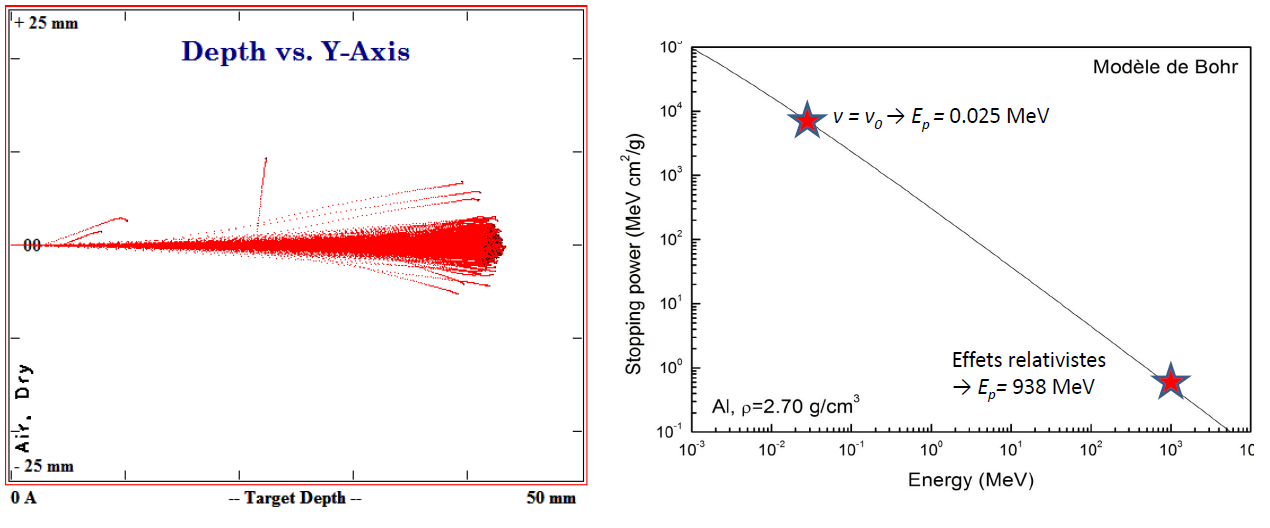
\includegraphics[scale=0.3]{ch2/image1.png}
	\captionof{figure}{ }
	\end{wrapfigure}
Ci-contre, à gauche, sont représenté les trajectoires de particules $\alpha$ d'une énergie
de 5.5 MeV. On observe que trois d'entre-elles sont rentrées en collisions avec les noyaux
(déviation angulaire plus importante). A droite, considérons un proton incident sur 
de l'aluminium, décrit par le modèle de Bohr. Ce modèle étant classique, il ne peut pas être
correct dans la zone relativiste. Lorsque la vitesse du projectile se rapproche de $v_0$, 
la vitesse de Bohr\footnote{On associe l'énergie à une certaine vitesse via l'énergie cinétique.}, 
on ne peut plus considérer que la particule est au repos, le modèle n'est dès lors plus 
valable\footnote{L'hypothèse de Bohr est telle que la particule cible est au repos.}

\section{Modèle semi-classique du pouvoir d'arrêt électronique}
Un rappel sur les oscillateurs classiques et l'approximation dipolaire est faite dans les
slides 5 à 12 : n'étant que des rappels/pré-requis, ils ne sont pas repris ici.

\subsection{Vitesses intermédiaires : $v_0\ll v \ll c$}
Dans le modèle semi-classique de \textsc{Bethe} (\textit{1930}), le noyau est traité 
classiquement et les électrons quantiquement, ils ne sont plus traités comme des oscillateurs
classiques. On s'intéresse ici au cas ou le modèle de Borh est correct. \\

Considérons un atome cible avec $Z_2$ électrons (masse $m$) et les états stationnaires $\ket j$ 
d'énergie $\epsilon_j$ où $j$ est un nombre quantique tel que $j=0$ dénote l'état fondamental. 
Les fréquences de résonance pour un atome dans son état initial sont données par
\begin{equation}
\hbar\omega_{j0}=\epsilon_j-\epsilon_0
\end{equation}
On dira que les électrons sont au repos durant l'interaction si $v\gg v_0$.
\\

Pour une énergie $Q$ perdue par l'ion incident, \textsc{Bethe} a posé
\begin{equation}
S=\sum_j\int Q d\sigma_Rf_{j0}(Q)
\end{equation}
où $\sigma_R$ est la section efficace de \textsc{Coulomb} pour un transfert d'énergie $Q$ 
(où $R$ pour \textsc{Rutherford}) et $f_{j0}$ sont les \textit{forces d'oscillateur généralisées}
qui incluent tous les effets quantiques pour la section efficace d'arrêt : ils décrivent les 
probabilités de transition entre les états pour une énergie transférée $Q$ donnée.\\

Afin de déterminer l'expression de $f_{j0}$, résolvons l'équation de Schrödinger dépendante du 
temps (celle-ci gouverne le mouvement électronique)
\begin{equation}
(H+V)\Psi(\overrightarrow{r},t)=i\hbar \frac{d\Psi(\overrightarrow{r},t)}{dt}
\end{equation}
où $H$ est l'hamiltonien d'un atome isolé de la cible, $\Psi(t)$ la fonction d'onde d'un état
lié et $V$ le potentiel décrivant l'interaction avec le projectile donné par
\begin{equation}
V(\overrightarrow{r},t)=\sum_{\nu=1}^{Z_2}\frac{-e_1e}{\overrightarrow{r}_\nu-\overrightarrow{R}(t)}
\end{equation}
où $\vec r = (\vec{r}_1,\dots \vec{r}_{Z_2})$ représente la trajectoire du projectile avec 
$\vec r_\nu$ l'opérateur position du $\nu^e$  électron et $\vec{R}=\vec{p}+\vec{v}t$. Développons
$\Psi(t)$ sur la base formée des états stationnaires
\begin{equation}
\Psi(\overrightarrow{r},t)=\sum_{j}c_j(t)e^{-i\epsilon_jt}|j\rangle
\end{equation}
où $\ket j$ sont les solutions de $H\ket j = \epsilon_j\ket j$. Dans le cadre de la méthode des
perturbations au premier ordre, on peut développer les coefficients $c_j$ en puissance du 
potentiel perturbatif $V$
\begin{equation}
c_j(t) = \delta_{j0} + c^{(1)}_j(t) + c^{(2)}_j(t) + \dots
\end{equation}
avec $\delta$ le symbole de Kronecker et

\begin{eqnarray}
c_j^{(1)}(t)=\frac{1}{i\hbar}\int_{-\infty}^{t}dt'e^{i\omega_{j0}t'}\langle j|V(\overrightarrow{r},t')|0\rangle\\
c_j^{(2)}(t)= \left(\frac{1}{i\hbar}\right)^2\sum_k\int_{-\infty}^{t}dt'e^{i\omega_{jk}t'}\langle j|V(\overrightarrow{r},t')|k\rangle
\times \int_{-\infty}^{t'}dt''e^{i\omega_{k0}t''}\langle k|V(\overrightarrow{r},t'')|0\rangle
\end{eqnarray}
et ainsi de suite mais ici nous ne nous intéressons que aux coefficients $c_j^{(1)}(\infty)$ car
seul le premier ordre nous intéresses. Ceux-ci représentent les amplitudes de transition. 
Substituons $c_j^{(1)}(\infty)$ dans l'expression explicite du potentiel, prenons-en la 
transformée de \textsc{Fourier} et intégrons sur $t'$
\begin{equation}
c_j^{(1)}(\infty)=\frac{-e_1e}{i\pi\hbar}\int \overrightarrow{dq}\frac{e^{-i\overrightarrow{q}.\overrightarrow{p}}}{q^2}F_{j0}(\overrightarrow{q})\delta(\omega_{j0}-\overrightarrow{q}.\overrightarrow{v})
\end{equation}
où $\DS F_{j0}(\overrightarrow{q})=\left\langle j\left| \sum_{\nu=1}^{Z_2}e^{i\overrightarrow{q}.\overrightarrow{r_\nu}}\right| 0\right\rangle$. Notons $Q=\frac{\hbar^2q^2}{2m}$. Par le 
\textsc{Postulat IV} de la mécanique quantique, les probabilités de transitions sont données 
par
\begin{equation}
P_j(p)=\left| \langle j| \Psi(\infty)\rangle\right|^2
\end{equation}
Ce qui donne dans le cadre de la méthode des perturbations au premier ordre
\begin{equation}
P_j(p)=\left| c_j^{(1)}(\infty)\right|^2
\end{equation}
Pour que $c_j^{(1)}(\infty) \neq 0$ pour $\omega_{j0} < q\nu$, il faut que (condition sur $Q$)
\begin{equation}
\omega_{j0}^2<q^2v^2 \Rightarrow 2mv^2Q>(\epsilon_j-\epsilon_0)^2
\end{equation}

\subsubsection{Approximation des collisions distantes - Approximation dipolaire}
Afin d'obtenir notre expression de $f_{j0}$, nous allons devoir utiliser une approximation. 
Considérons $c_j^{(1)}(\infty)$ à grand $p$ (\textit{collisions distantes}). Par l'approximation
dipolaire
\begin{equation}
e^{i\overrightarrow{q}.\overrightarrow{r}}\simeq 1+i\overrightarrow{q}.\overrightarrow{r}
\end{equation}
On obtient donc
\begin{equation}
F_{j0}(\overrightarrow{q})\simeq i\overrightarrow{q}\left\langle j\left| \sum_{\nu=1}^{Z_2}\overrightarrow{r_\nu}\right| 0\right\rangle
\end{equation}
En choisissant l'axe $x$ selon la vitesse du projectile et l'axe $y$ selon le paramètre 
d'impact, on voit apparaître des fonctions de \textsc{Bessel} modifiée $K_{0,1}$, d'ordre 0 et 1
\begin{equation}
c_j^{(1)}(\infty)=-\frac{2e_1e\omega_{j0}}{i\hbar v^2}\left\langle j\left| \sum_{\nu}^{Z_2}\overrightarrow{r}_\nu \right|0\right\rangle
 \times\left(iK_0\left(\frac{\omega_{j0}p}{v}\right),K_1\left(\frac{\omega_{j0}p}{v}\right),0\right)
\end{equation}
Les probabilités de transitions deviennent donc (données par $|c_j|^2$)
\begin{equation}
P_j(p)=-\frac{2e_1^2e^2Z_2}{mv^2p^2\hbar\omega_{j0}}f_{j0}
 \times\left\{\left[\frac{\omega_{j0}p}{v}K_0\left(\frac{\omega_{j0}p}{v}\right)\right]^2+\left[\frac{\omega_{j0}p}{v}K_1\left(\frac{\omega_{j0}p}{v}\right)\right]^2\right\}
\end{equation}
La grandeur $f_{j0}$ est appelée la \textbf{force d'oscillateur dipolaire} et a comme
expression
\begin{equation}
f_{j0}=\frac{2m}{3\hbar^2Z_2}(\epsilon_j-\epsilon_0)\left|\left\langle j\left|\sum_{\nu}^{Z_2}\overrightarrow{r}_\nu\right|0\right\rangle\right|^2
\end{equation}
Avec la règle de somme de \textsc{Thomas-Reiche-Kuhn} $\sum_j f_{j0}=1$.

\subsubsection{Comparaison modèle classique et semi-classique}
Maintenant que nous avons la probabilité d'une transition, il nous faut l'énergie moyenne. 
Considérons l'énergie transférée moyenne $T_{moy}$
\begin{equation}
T_{moy}(p)=\sum_jP_j(p)\hbar\omega_{j0}
\end{equation}
Comparons cette expression avec le résultat classique donné par 
\begin{equation}
T= \frac{2e_1^2e^2}{mv^2p^2}f_{dist}(p),\qquad\text{ où }\quad 
f_{dist}(p)=\left[\frac{\omega_{0}p}{v}K_0\left(\frac{\omega_{0}p}{v}\right)\right]^2+\left[\frac{\omega_{0}p}{v}K_1\left(\frac{\omega_{0}p}{v}\right)\right]^2
\end{equation}
Les expressions sont identiques à condition que
\begin{equation}
f_{dist}(p)=\sum_jf_{j0}\left[\frac{\omega_{j0}p}{v}K_0\left(\frac{\omega_{j0}p}{v}\right)\right]^2+\left[\frac{\omega_{j0}p}{v}K_1\left(\frac{\omega_{j0}p}{v}\right)\right]^2
\end{equation}
Pour généraliser les fonctions $f_{j0}$ que nous venons d'élaborer aux grandes valeurs de $Q$, 
\textsc{Bethe} a posé
\begin{equation}
f_{j0}(Q)=\frac{1}{Z_2}\frac{\epsilon_j-\epsilon_0}{Q}|F_{j0}(\overrightarrow{q})|^2
\end{equation}
Avec cette forme la, lorsque $Q$ est petit, on retrouve l'expression que nous venons de calculer
\begin{equation}
f_{j0}(Q)\big\vert_{Q\simeq 0}=f_{j0}
\end{equation}

\subsubsection{Pouvoir d'arrêt : formule de Bethe}
Il est nécessaire de faire la distinction entre les collisions distantes ou proche (via $p$), soit 
les collision avec une grande ou petite quantité de mouvement transférée (via $q$) ou encore 
les collisions avec une grande ou petite énergie transférée (via $Q$). Pour se faire, 
nous allons séparer l'intégrale suivante en deux parties par rapport à $Q_0$
\begin{equation}
S=\sum_j\int Q d\sigma_Rf_{j0}(Q)
\end{equation}
$\bullet$ Pour $Q<Q_0$, l'approximation dipolaire est valide ($Q_0$)
\begin{equation}
S_{dist}=\sum_jf_{j0}\int_{(\epsilon_j-\epsilon_0)^2/2mv^2}^{Q_0} Q d\sigma_R
\end{equation}

$\bullet$ Pour $Q>Q_0$, il faut déterminer la borne supérieure de l'intégrale. On considère que 
la masse d'un ion $m_1\gg m$, la masse d'un électron.
\begin{equation}
T_{max} = \gamma E = \frac{4m_1m}{(m_1+m)^2}\frac{m_v^2}{2} \approx 2mv^2
\end{equation}
où nous avons négliger $m$ par rapport à $m_1$. On trouve alors la section efficace 
d'arrêt suivante
\begin{equation}
S_{proche}=\int_{Q_0}^{2mv^2} Q d\sigma_R\sum_jf_{j0}(Q)
\end{equation}
\textsc{Bethe} a démontré que
\begin{equation}
\sum_jf_{j0}(Q)=1
\end{equation}
Nous avons alors
\begin{equation}
S_{proche}=\int_{Q_0}^{2mv^2} Q d\sigma_R\equiv \sum_jf_{j0}\int_{Q_0}^{2mv^2} Q d\sigma_R
\end{equation}
En sommant les collisions proches et distantes, on trouve finalement
\begin{equation}
S=S_{proche}+S_{dist}= \sum_jf_{j0}\int_{(\epsilon_j-\epsilon_0)/2mv^2}^{2mv^2} Q d\sigma_R
\end{equation}
En considérant l'expression explicite $d\sigma_R= 2\pi \frac{e_1^2e_2^2}{m_2v^2}\frac{dQ}{Q^2}$, 
on obtient
\begin{equation}
S=\frac{4\pi e_1^2e^2}{mv^2}Z_2\sum_jf_{j0}\ln{\frac{2mv^2}{\epsilon_j-\epsilon_0}}
\end{equation}
La formule du pouvoir d'arrêt de \textsc{Bethe} se note généralement\\

\cadre{\begin{equation}
S_{e}=\frac{4\pi e_1^2e^2}{mv^2}Z_2\ln{\frac{2mv^2}{I}}
\end{equation}
où $I$ est définie comme l'énergie moyenne d'excitation telle que $\ln I=\sum_j f_{j0}\ln{
(\epsilon_j-\epsilon_0)}$. Ceci n'est valable que \textbf{si} $m_1\gg m, v\gg v_0 \to mv^2 \gg
 \hbar \omega_0$.}\ \\
 
On peut facilement comparer le modèle de \textsc{Bethe} à celui de \textsc{Bohr} via 
\begin{equation}
S_e=\frac{4\pi Z_2 e_1^2e^2}{mv^2}L_e
\end{equation}
où 
\begin{equation}
L_e=\ln\frac{Cmv^3}{|e_1e|\omega_0}
\end{equation}
pour le \textsc{Bohr} et 
\begin{equation}
L_e=\ln{\frac{2mv^2}{I}}
\end{equation}
pour \textsc{Bethe}.

\subsubsection{Dépendances principales du pouvoir d'arrêt}
Le pouvoir d'arrêt se compose lui-même de trois dépendances\ \\

\retenir{\begin{equation}
-\left( \frac{dE}{dx}\right)_{elec}=NS_{e}=\frac{4\pi e_1^2e^2}{mv^2}NZ_2\ln{\frac{2mv^2}{I}}
\end{equation}}\ \\

Les dépendances sont les suivantes
\begin{enumerate}
\item $\frac{4\pi e_1^2e^2}{mv^2}\Rightarrow{\mbox{D\'ependance principale dans la vitesse}}$, plus la vitesse augmente, plus le pouvoir d'arrêt diminue.
\item $NZ_2\Rightarrow{\mbox{D\'ependance principale dans le mat\'eriau}}$, plus il est grand, plus le pouvoir augmente.
\item $\ln{\frac{2mv^2}{I}}\Rightarrow{\mbox{D\'ependance faible dans la vitesse et dans le mat\'eriau}}$
\end{enumerate}

	\subsubsection{Énergies moyenne d'excitation}
	\begin{wrapfigure}[7]{r}{6.5cm}
	\vspace{-5mm}
	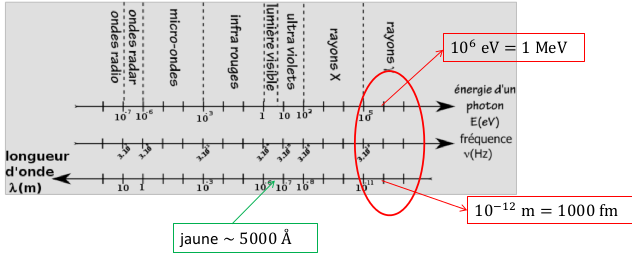
\includegraphics[scale=0.5]{ch2/image2.png}
	\captionof{figure}{ }
	\end{wrapfigure}
	

L'énergie moyenne d'excitation $I$ ne dépend \textbf{que} du matériau et \textbf{pas} du 
projectile. Il est possible de le calculer mais tout le monde s'en fiche car on peut l'obtenir
expérimentalement\footnote{De plus, comme il intervient dans $\log S$ il n'est pas nécessaire
de connaître sa valeur avec précision} via des formules empiriques. Celui-ci varie approximativement
linéairement (les irrégularités sont dues à la structure en couches de l'atome) avec $Z$ :
\textit{modèle de l'atome de Thomas-Fermi} où les électrons atomiques forment un gaz.

\newpage
\subsection{Grandes vitesses - Équation de \textsc{Bethe-Bloch} : $v_0<v\approx c$}
\textsc{Bloch} a apporté de nombreuses corrections à l'équation de \textsc{Bethe} pour 
former l'équation de \textsc{Bethe-Block}\\

\cadre{\begin{equation}
S_e = \dfrac{4\pi r_e^2mc^2}{\beta^2}Zz^2L(\beta)
\end{equation}
où $\DS L(\beta)= L_0(\beta) = \frac{1}{2}\ln\left(\frac{2mc^2\beta^2W_m}{1-\beta^2}\right)
-\beta^2-\ln I-\frac{C}{Z}-\frac{\delta}{2}$.}\ \\

Il s'agit en réalité de la même équation mais notée différemment, toute la différence se 
trouve dans le \textit{stopping number} $L$ qui contient donc les termes correctifs. 
Intéressons-nous à ceux-ci
\begin{itemize}
\item[$\bullet$] \textit{Corrections dues aux collisions}\ \\
$W_m$ donne l'énergie maximale transférée en une collision à un électron
libre\footnote{Il s'agit d'une expression relativiste non-approchée}
\begin{equation}
W_m=\frac{2mc^2\beta^2}{1-\beta^2}\left[1+\frac{2m}{m_1(1-\beta^2)^{1/2}}+\left(\frac{m}{m_1}\right)^2\right]^{-1}
\end{equation}
Pour $m_1\gg m$, on retrouve bien $2m\gamma_1^2v^2$.
\item[$\bullet$] \textit{Corrections relativistes}\ \\
Si $v\approx c$, il faut apporter des corrections relativistes. Lorsque l'on travaille avec
des vitesses relativistes, il faut considérer des électrons de plus en plus lointain ce qui, 
forcément, augmente le pouvoir d'arrêt. En effet, $p_{max} \propto \gamma_1v/\omega_0$ ce qui
montre que le paramètre d'impact augmente lorsque la vitesse fait de même. Le calcul relativiste
classique du champ donne
\begin{equation}
\overrightarrow{E}(\omega)=-\frac{e_1\omega}{\pi \gamma_1v^2}\left(\frac{i}{\gamma_1}K_0\left(\frac{\omega_{j0}p}{\gamma_1v}\right),K_1\left(\frac{\omega_{j0}p}{\gamma_1v}\right),0\right)
\end{equation}
On y voit apparaître des $\gamma_1$ et $f(p)$ se voit modifiée par ce fameux terme
\begin{equation}
f_{dist}(p)=\frac{1}{\gamma_1^2}\left[\frac{\omega_{0}p}{\gamma_1v}K_0\left(\frac{\omega_{0}p}{\gamma_1v}\right)\right]^2+\left[\frac{\omega_{0}p}{\gamma_1v}K_1\left(\frac{\omega_{0}p}{\gamma_1v}\right)\right]^2
\end{equation}
La composante principale en la vitesse se voit modifiée
\begin{equation}
\frac{4\pi e_1^2e^2}{mv^2}\Rightarrow \frac{4\pi e_1^2e^2}{m\gamma_1^2v^2}=\frac{4\pi e_1^2e^2}{mv^2}(1-\beta^2)
\end{equation}
où le $(1-\beta^2)$ apparaissant permet de comprendre le terme correspondant dans la formule de 
\textsc{Bethe-Bloch}, il va être possible de lui donner un sens physique. Sachant que la quantité 
de mouvement de la particule incidente devient $m\gamma_1v$, on en tire
\begin{equation}
T_{max}=2m\gamma_1^2v^2
\end{equation}
La composant logarithmique se modifie selon
\begin{equation}
\ln{\frac{2mv^2}{I}}\Rightarrow \ln{\frac{2m\gamma_1^2v^2}{I}}=\ln{\frac{2mv^2}{I(1-\beta^2)}}
\end{equation}
La combinaison de toutes ces relations implique donc que le pouvoir d'arrêt augmente lorsque 
la vitesse augmente, ce qui est la conséquence du traitement relativiste. 
\end{itemize}

\newpage

\begin{itemize}
\item[$\bullet$] \textit{Correction de densité}\ \\
Le terme correspondant à ces corrections est le $-\delta/2$. La formule de \textsc{Bethe} est 
valable pour un gaz de faible densité (atomes isolés) mais pour un solide il faut tenir compte
des effets collectifs d'un grand nombres d'atomes : on peut utiliser le modèle de Fermi. Une 
particule chargée incidente va polariser le milieu. Le champ électrique induit va alors donner un
moment dipolaire électrique aux atomes et il en résultera un champ électrique opposé à celui 
produit par la particule chargée. Le champ électrique sera donc réduit via l'écrantage des dipôles.\\

A cause de cette diminution du champ (à cause de la polarisation), les atomes lointains ont un 
effet plus faible. L'effet de densité apparaît surtout aux grandes vitesses, en même temps que les 
effets relativiste (ils vont se "compenser"). S'il n'est signifiant qu'aux énergies élevées c'est 
à cause du facteur $\gamma_1$ présent dans $p_{max}$ qui augmente l'erreur commise en ignorant la
polarisation du milieu : si $v$ augmente, $p_{max}$ augmente et donc $\delta/2$ augmente causant une
diminution de $S$.

\begin{center}
	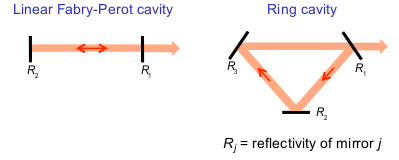
\includegraphics[scale=0.5]{ch2/image3.png}
	\captionof{figure}{L'effet relativiste et de densité vont se stabiliser de sorte que le 
	pouvoir d'arrêt devient constant. On parle alors de \textit{plateau de Fermi}, constant à
	grande vitesse.}
\end{center}

On peut écrire la correction de densité
\begin{equation}
\frac{\delta}{2}=\ln{\frac{\hbar\omega_p}{I}}+\ln{\gamma_1\beta}-\frac{1}{2}
\end{equation}
avec $\omega_p=\sqrt\frac{ne^2}{\epsilon_0m}$ la \textit{pulsation plasma}, mais ceci est plus
informatif.

\item[$\bullet$] \textit{Correction shell} ("en couches")\ \\
Il s'agit du terme $-C/Z$. Nos deux formules sont basées sur l'hypothèse que $v\gg v_0$ (permet
de calculer $I$ moyen). Lorsque que n'est plus le cas, on ne peut plus considérer que tous les
électrons ont la même énergie de liaison. Le problème est que certains électrons sont plus liés 
que d'autres. Comme ils seront plus durs à arracher, leur contribution au pouvoir d'arrêt va 
diminuer et il ne faudra plus les considérer. On ajoute ainsi un terme de correction "moyen" qui
réduit $S$ de maximum 6\% qui ne dépend que de la vitesse et du matériau considéré, peu importe 
les couches. Il existe deux méthodes pour calculer $C/Z$
	\begin{enumerate}
	\item Une basées sur les fonctions d'ondes hydrogénoïdes (HWF)\footnote{Un électron interne ne
	 peut
	 pas être représenté par une fonction d'onde de la sorte mais comme la rigueur absolue n'est 
	 pas possible en s'en contentera car \textit{au moins} on a un résultat, bien que moins 
	 rigoureux.}
	\item Une basée sur l'approximation en densité locale (LDA)
	\end{enumerate}
	
%\begin{center}
\hspace{-1cm}	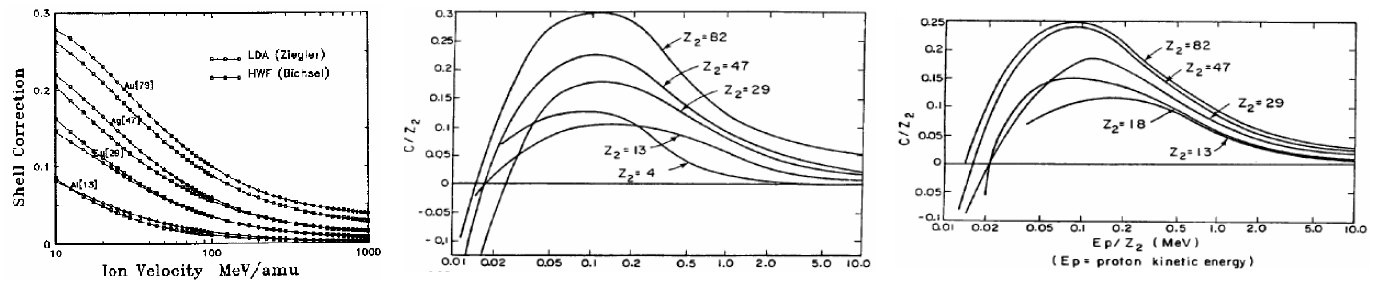
\includegraphics[scale=0.4]{ch2/image4.png}
	\captionof{figure}{A gauche la comparaison théorie/expérience (relativement bonne et comme la
	correction est logarithmique on s'en contentera), au centre le calcul par la méthode LDA et à
	droite selon HWF. L'écart entre les méthodes est plus grand pour des $Z$ élevés mais 
	les deux sont globalement assez bonnes.}
%\end{center}
\end{itemize} \ \\

Il est possible d'aller encore plus loin et de considérer des corrections au-delà de l'approximation
de \textsc{Born} au premier ordre.  On va considérer des vitesses toujours plus grande que $v_0$ mais
très proche de celle-ci de sorte que l'approximation de Born n'est plus valable\footnote{Il faut 
en effet que $v\gg v_0$ pour que $L_0$ soit valable}.Il faut rajouter des termes correctifs à 
$L_0$ qui apparaissent lors d'un développement de $L$ en puissance de $z$\ \\

\cadre{\begin{equation}
L(\beta) =  L_0(\beta) + zL_1(\beta) + z^2L_2(\beta)
\end{equation}}\ \\

Passons à nouveau en revue les différentes corrections
\begin{itemize}
\item[$\bullet$] \textit{Correction de Barkas-Andersen}\ \\
Il s'agit du terme $zL_1(\beta)$. Il s'agit d'une proportionnalité à une puissance impaire de la 
charge. Si la charge est positive, cela attire le nuage d'électrons et il y aura plus d'interactions :
augmentation du pouvoir d'arrêt. Si la charge est négative, les électrons sont repoussés et le 
pouvoir d'arrêt diminue. $S$ diffère donc entre les particules et antiparticules.
\begin{center}
	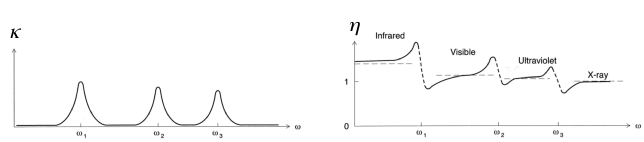
\includegraphics[scale=0.5]{ch2/image5.png}
	\captionof{figure}{Protons et antiprotons incidents sur une cible de silicium : le pouvoir 
	d'arrêt est plus important pour les protons que pour des antiprotons.}
\end{center}
\item[$\bullet$] \textit{Correction de Bloch}\ \\
Il s'agit du terme $z^2L_2(\beta)$, une correction pas très importante que l'on évalue généralement
avec l'évaluation de \textsc{Bichsel}
\begin{equation}
z^2L_2(y) = -y^2[1.202-y^2(1.042-0.855y^2+0.343y^4)]
\end{equation}
où $y=z\alpha/\beta$ avec $\alpha = 1/137$ le constante de structure fine.
\end{itemize}

\newpage
	\begin{wrapfigure}[11]{r}{9cm}
%	\vspace{-5mm}
	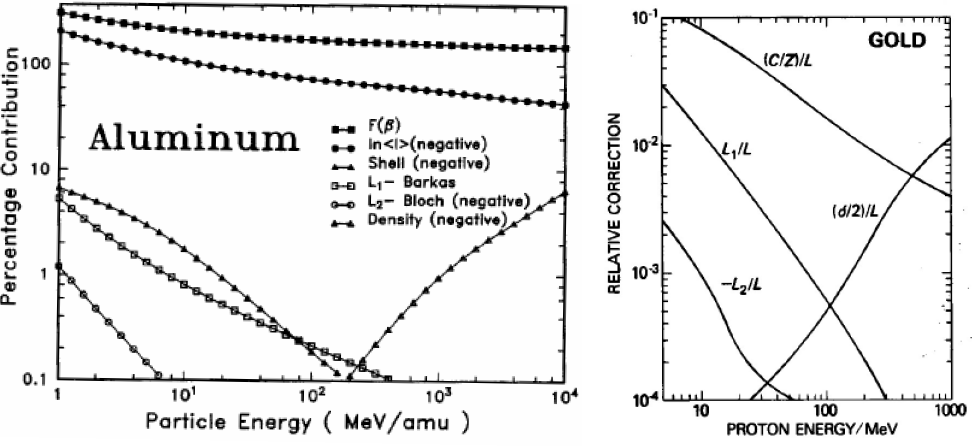
\includegraphics[scale=0.4]{ch2/image6.png}
	\captionof{figure}{ }
	\end{wrapfigure}
Évaluons maintenant les effets des différentes corrections. Le graphique ci-contre (à gauche) 
concerne des protons incidents sur une cible d'aluminium. On peut y voir que la correction de
\textsc{Bloch} (en bas à gauche) est vraiment très faible. A droite est représenté la correction
relative pour des protons incidents sur une cible d'or ($L_1$ concerne \textsc{Barkas} et $L_2$
\textsc{Bloch}).


\subsection{Petites vitesses}
Lorsque $v \lesssim v_0$, on ne peut plus appliquer la méthode des perturbations et il faut 
commencer à prendre en compte les captures électroniques par l'ion indicent (l'ion va si
lentement qu'il peut capturer un (ou plusieurs) électron) modifiant la charge $z^*$ de 
celui-ci. Par la théorie de \textsc{Thomas-Fermi}
\begin{equation}
z^*=z\left(1-e^{-v/(z^{2/3}v_0)}\right)
\end{equation}
Une technique consiste à considérer un état de charge moyen même si ce n'est pas vrai en tout 
point.


\section{Pouvoir d'arrêt nucléaire (faibles vitesses)}
Les effets étant tellement négligeable que nous ne rentrerons pas dans les détails ici. Comme
vu au premier chapitre, les collisions nucléaire pour des ions incidents sont rares et contribuent
peu au pouvoir d'arrêt total. Elle se produise presque exclusivement pour des ions incidents de 
faible vitesse et même alors leur contribution est faible. Cependant, elle peuvent avoir des effets
à postériori et causer des dégâts radiatifs.\\

	\begin{wrapfigure}[12]{r}{5.6cm}
	\vspace{-11mm}
	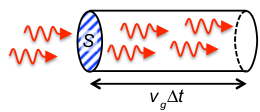
\includegraphics[scale=0.34]{ch2/image7.png}
	\captionof{figure}{ }
	\end{wrapfigure}
Plaçons-nous dans le système du centre de masses pour observer la diffusion par un angle 
$\theta$ due à un potentiel central $V(r)$. Reprenons la formule générale pour la section efficace
d'arrêt 
\begin{equation}
S_n = \int Td\sigma = \int T 2\pi p dp = 2\pi\gamma E\int \sin^2(\theta/2)pdp
\end{equation}
où $\gamma = \frac{4m_1m_2}{(m_1+m_2)^2}$. Pour le calculer, il est nécessaire de connaître $\theta$
ce qui peut se faire avec le schéma avec une particule incidente et cible représenté ci-contre.\\

Pour évaluer $\theta$, on utilise l'équation de la variation angulaire en coordonnée sphérique tout
en introduisant le potentiel. 

\begin{eqnarray*}
\frac{m_0}{2}\left[ \left( \frac{dr}{dt}\right)^2+r^2\left( \frac{d\varphi}{dt}\right)^{2}\right]+V(r)=\frac{m_0}{2}v^2\equiv E_r\\
m_0r^2\frac{d\varphi}{dt}=-m_0pv
\end{eqnarray*}
On en tire
\begin{equation}
\theta=\pi-2\int_{r_{m}}^\infty dr \frac{p}{r^2}\left( 1-\frac{V(r)}{E_r}-\frac{p^2}{r^2}\right)^{-1/2}
\end{equation}


Il faut maintenant spécifier le potentiel. Le plus logique serait d'utiliser celui de \textsc{Coulomb}
mais sa variation en $1/r$ cause une divergence du paramètre d'impact à cause de la portée infinie. 
Comme il y a toujours interaction, on va préférer considérer un effet d'écrantage par les électrons
atomiques qui diminue la portée du potentiel. Pour se faire, on va simplement introduire une 
exponentielle décroissante $\exp(-r/r_s)$.\\

Pour un modèle plus précis, on peut insérer une fonction $F_s(r/r_s)$. Le potentiel d'interaction 
devient alors
\begin{equation}
V(r)=\frac{z_1Z_2e^2}{r}F_s(\frac{r}{r_s})
\end{equation}
Il s'agit de la \textit{fonction d'écrantage universelle}, obtenue par ajustement aux résultats 
expérimentaux.\\

	\begin{wrapfigure}[12]{r}{5.6cm}
	\vspace{-11mm}
	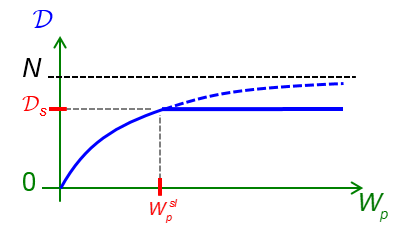
\includegraphics[scale=0.34]{ch2/image8.png}
	\captionof{figure}{ }
	\end{wrapfigure}
Mettons maintenant ces effets ensemble en considérant des protons incidents sur une cible 
d'aluminium comme représenté ci-contre. Nous avons $S = S_{elec} + S_{nucl} \approx S_{elec} 
= S_{coll}$. On voit que l'effet du pouvoir d'arrêt nucléaire est très faible, on retrouve
le plateau de Fermi à grande vitesse et une pente ou la formule de \textsc{Bohr} est valable.


\section{Pouvoir d'arrêt massique électronique et influence de la phase}
Par définition, le pouvoir d'arrêt massique d'un matériau est le rapport du pouvoir d'arrêt 
linéique et de lamasse volumique $\rho$ de ce matériau (unités usuelle : MeV.cm$^2$.g$^{-1}$. 
\begin{equation}
\frac{NS(E)}{\rho}=-\frac{1}{\rho}\frac{dE}{dx}
\end{equation}
Comme $\rho = M_AN/N_A$ où $M_A=AM_u$, en divisant des deux côtés par cette même quantité on 
trouve\\

\cadre{\begin{equation}
-\dfrac{1}{\rho}\dfrac{dE_{elec}}{dx} = 4\pi r_e^2mc^2\frac{N_A}{M_u}\dfrac{Z}{A}\dfrac{z^2}{\beta^2}
L(\beta)
\end{equation}}\ \\

Passons en revue les quatre facteurs du pouvoir d'arrêt massique électronique
\begin{enumerate}
\item Le facteur constant $4\pi r_e^2mc^2N_A/M_u = 0.307$ MeV.cm$^2$.g$^{-1}$ qui donne l'ordre
de grandeur de ce pouvoir
\item Le facteur $Z/A$ compris entre 0.4 et 0.5 pour tout les isotopes stable (sauf $H$). Comme
c'est le terme principal de dépendance du matériau et que celui-ci est $\pm$ constant la dépendance
du matériau est faible : c'est l'intérêt de cette formule
\item Le facteur $\beta^{-2}$ est une fonction monotone décroissante de la vitesse de l'ion qui
tend vers 1 pour les grandes énergies. Ce-dernier explique la diminution du pouvoir d'arrêt 
avec l'énergie. 
\item Le nombre d'arrêt $L(\beta)$ est une fonction monotone croissante (lente) de la vitesse 
et de $Z$.
\end{enumerate}

\subsection*{Influence de la phase}
Aux grandes énergies, la correction de densité influe impliquant une grande correction de phase 
dans les solides et faible dans les gaz. Aux faibles énergies il faut tenir compte de l'influence
des liaisons chimiques et intermoléculaires ce qui se traduit par une modification de la
valeur de $I$.

\section{Parcours et courbe de Bragg} 
\subsection{Parcours}
Lorsque les particules \textbf{chargées} perdent leur énergie dans la matière, elles parcourent une
certaine distance dans la matière mais celle-ci peut être variable a cause des pertes d'énergies 
et des déviations aléatoires (\textit{starggling}). Il faut alors définir plusieurs parcours
\begin{itemize}
\item[$\bullet$] Le parcours $R$ d'une particule chargée d'énergie $E$ dans un milieu et 
la valeur moyenne $\langle l \rangle$ de la longueur $m$ de sa trajectoire suivie jusqu'à son 
arrêt (en négligeant le mouvement thermique)
\item[$\bullet$] Le parcours projeté $R_p$ d'une particule chargée d'énergie $E$ dans un milieu. 
Celui-ci correspond à la valeur moyenne de sa profondeur de pénétration $\langle d \rangle$ dans la
direction initiale de la particule.
\end{itemize}
A cause du caractère sinueux des trajectoires, $R_r<R$. On défini alors le \textbf{facteur de détour}
$R_p/R_{CSDA} < 1$.\\

Dans l'approximation $CSDA$
\begin{equation}
R_{CSDA}=\int^{E}_{0}\frac{dE'}{NS(E')}
\end{equation}
En remplaçant $S$ par l'expression de \textsc{Bethe} (non-relativiste, avec $dE=Mv$d$v$)
\begin{equation}
R_{CSDA}\propto \int^{v}_{0}\frac{v^3dv}{L(v)}
\end{equation}
En négligeant la dépendance en la vitesse du nombre d'arrêt 
\begin{equation}
R_{CSDA}\propto v^4\propto E^2
\end{equation}
En réalité, l'équation de \textsc{Bethe} (ou \textsc{Bethe-Bloch}) n'est pas valable à faibles
vitesses et il faut nécessairement passer par de faibles vitesses pour s'arrêter. On utilisera 
alors la formule empirique suivante
\begin{equation}
\rho R_{CSDA}=\frac{E^{1.77}}{415}+\frac{1}{670}
\end{equation}

\subsubsection{Considérations sur le parcours}
Reprenons l'approximation $NS(E)\propto 1/E$. Soit une particule incidente de masse $M_i$ et de
charge $z_i$
\begin{equation}
NS(E)=-\frac{dE}{dx} \Rightarrow -\frac{M_i}{z_i^2}\frac{dv^2}{dx}\propto \frac{1}{v^2}
\end{equation}
Pour deux particules incidentes $(M_1,z_1)$ et $(M_2, z_2)$ de même vitesse initiale
\begin{equation}
\frac{R_{CSDA}^1}{R_{CSDA}^2}=\frac{M_1z_2^2}{M_2z_1^2}
\end{equation}
Il s'agit d'une petite formule utile pour estimer l'ordre de grandeur qui nous informe que le range
pour des protons et des $\alpha$ de même vitesse est similaire.


\subsection{Courbes de Bragg}
Soit un milieu semi-infini et un faisceau parallèles de particules chargées identiques et de même
énergie : toutes les particules vont forcément s'arrêter, après une distance $R_{CSDA}$. La 
courbe de \textsc{Bragg} donne la \textbf{dose} (énergie moyenne déposée par unité de masse de la
cible) déposée par la particule chargée en fonction de la profondeur. \\

A une profondeur $x$, la particule doit encore parcourir $d=R_{CSDA}-x$. Comme l'énergie déposée
$D \propto S \propto 1/v^2$, cela implique que $R_{CSDA}\propto v^4$. Dès lors
\begin{equation}
D\propto \frac{1}{\sqrt d}=\frac{1}{\sqrt{R_{CSDA}-x}}
\end{equation}

	\begin{wrapfigure}[12]{r}{8.5cm}
	\vspace{-7mm}
	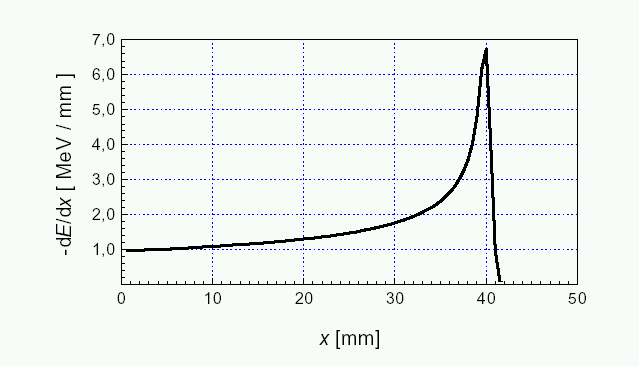
\includegraphics[scale=0.5]{ch2/image9.png}
	\captionof{figure}{Protons de 700 MeV dans de l'eau}
	\end{wrapfigure}
Ceci a des applications en protonthérapie (ou hadronthérapie). Lorsque l'on a une tumeur, il faut
la soumettre à un rayonnement pour l'éliminer. On pourrait envoyer des électrons, mais entre la 
tumeur et la peau il y a pas mal de choses qu'il ne vaut mieux pas endommager et le problème est que 
les électrons vont déposer pas mal d'énergie entre les deux. Avec la protonthérapie, la zone dans 
laquelle il ne faut pas déposer l'énergie sera faible et le maximum d'énergie sera déposé la ou 
la tumeur se situe.\\

\subsection*{Interactions nucléaires fortes}
	\begin{wrapfigure}[5]{l}{3cm}
	\vspace{-7mm}
	
\includegraphics[scale=1.5]{ch2/image10.png}
%M	\captionof{figure}{ }
	\end{wrapfigure}
Lorsqu'un ion s'approche très près d'un noyau, une interaction nucléaire forte est possible et le
noyau peut être brisé. Par exemple, en fragmentant le plomb on aura un excès de neutron. Ce 
processus de production de neutrons est nomme \textit{spallation}. Le projet \textit{Myrrha} se
base la dessus. L'idée est de faire un réacteur avec un accélérateur en envoyant des protons sur
du Pb pour produire des neutrons et après se trouve un réacteur classique : pour l'arrêter, il suffit
de couper l'accélérateur.